\documentclass[notheorems]{beamer}
%\documentclass[handout]{beamer}
%\documentclass[handout,notes=show]{beamer}

\usetheme{metropolis}
%\usecolortheme{dolphin}
% No navigation bars
\beamertemplatenavigationsymbolsempty

\usepackage{amsmath, amssymb, amsfonts, tikz}
\usepackage[utf8]{inputenc}
\usepackage[T1]{fontenc}
\usepackage[english]{babel}

\usepackage{tcolorbox}
\tcbuselibrary{theorems}

\usepackage{cleveref}
\usepackage{amsthm}
\theoremstyle{plain}

\tcbset{
defstyle/.style={fonttitle=\bfseries\upshape,% fontupper=\slshape,
arc=0mm, %colback=blue!5!white,colframe=blue!75!black
theorem name,
},
thmstyle/.style={fonttitle=\bfseries\upshape, fontupper=\slshape,
colback=red!10!white,colframe=red!75!black,
theorem name,
},
}
\newtcbtheorem[number within=section,crefname={definition}{definitions}]%
{definition}{Definition}{defstyle}{def}
\newtcbtheorem[number within=section,crefname={theorem}{theorems}]%
{theorem}{Theorem}{thmstyle}{thm}
\newtcbtheorem[number within=section,crefname={example}{examples}]%
{example}{Example}{defstyle}{ex}
\newtcbtheorem[number within=section,crefname={question}{questions}]%
{question}{Question}{defstyle}{que}
\newtcbtheorem[number within=section,crefname={observation}{observations}]%
{observation}{Observation}{defstyle}{obs}
%\newtheorem{theorem}{Theorem}[section]
%\newtheorem{corollary}[theorem]{Corollary}
%\newtheorem{lemma}[theorem]{Lemma}
%\newtheorem{algorithm}[theorem]{Algorithm}
%\newtheorem{proposition}[theorem]{Proposition}
%\newtheorem{claim}[theorem]{Claim}
%\newtheorem{fact}[theorem]{Fact}
%\newtheorem{conjecture}[theorem]{Conjecture}
%% Definition-like environments, normal text
%% Numbering is in sync with theorems, etc
%\theoremstyle{definition}
%\newtheorem{definition}[theorem]{Definition}
%% Remark-like environments, normal text
%% Numbering is in sync with theorems, etc
%\theoremstyle{definition}
%\newtheorem{remark}[theorem]{Remark}
%\newtheorem{observation}[theorem]{Observation}
%% Example-like environments, normal text
%% Numbering is in sync with theorems, etc
%\theoremstyle{definition}
%\newtheorem{example}[theorem]{Example}
%\newtheorem{question}[theorem]{Question}
\DeclareMathOperator{\sgn}{sgn}
\newcommand{\terminology}[1]{\textbf{#1}}

\newcommand{\NN}{\mathbb{N}}
\newcommand{\ZZ}{\mathbb{Z}}
\newcommand{\QQ}{\mathbb Q}
\newcommand{\RR}{\mathbb R}
\newcommand{\lt}{<}
\newcommand{\gt}{>}
\newcommand{\amp}{&}

\usepackage{enumitem}



\author{Alex J. Best}
\institute{VU Master Seminar - Algebra}
\date{10/10/22}
\title{The (inescapable) $p$-adics}

\begin{document}

\maketitle

%\begin{frame}
%\frametitle{Table of Contents}
%\tableofcontents[currentsection]
%\end{frame}

\begin{frame}{Linear recurrence sequences}
    \begin{definition}{Linear recurrence sequence}{linrec}
        A \terminology{linear recurrence sequence}, is a sequence whose \(n\)th term is a linear combination of the previous \(k\) terms (for all \(n \ge k\)).
    \end{definition}

    \only<2-3>{\begin{example}{Fibonacci}{example-27}
            \(a_0 = 0, a_1 = 1\) and \(a_{n} = a_{n-1} + a_{n-2}\) for \(n \ge k =2\):
            \begin{equation*}
                0, 1, 1, 2, 3, 5, 8, 13, 21, 34, 55, 89, 144, 233, 377, 610, 987, 1597, 2584, 4181, 6765, 10946, 17711, 28657, 46368, 75025, 121393, 196418, 317811, 514229, 832040, 1346269, 2178309, 3524578, 5702887, 9227465, 14930352, 24157817, 39088169, 63245986, 102334155, \ldots\text{.}
            \end{equation*}
            \only<3>{\(a_n\) grows exponentially.}
            %
    \end{example}}

    \only<4-5>{\begin{example}{A periodic sequence}{example-28}
            \(a_0 = 1, a_1 = 0\) with \(a_n = -a_{n-1} - a_{n-2}\)
            \begin{equation*}
                1,0,-1,1,0,-1,1,0,-1,1,0,-1,1,0,-1,1,0,-1,1,0,-1,1,0,-1,1,0,-1,\ldots\text{.}
            \end{equation*}
            \only<5>{\(a_n\) is periodic now.}
        \end{example}
    }
    \only<6-7>{\begin{example}{Natural numbers interlaced with zeroes}{example-29}
            \(a_0= 1,a_1=0,a_2 = 2,a_3= 0\) with \(a_n = 2a_{n-2} - a_{n-4}\)%
            \begin{equation*}
                1,0,2,0,3,0,4,0,5,0,6,0,7,0,8,0,9,0,10,0,11,0,12,0,13,0,14,0,15,0,16,0,17,0,\ldots
            \end{equation*}
            \only<7>{not periodic but the zeroes \emph{do} have a regular repeating pattern.}
    \end{example}}
\end{frame}

\begin{frame}{The ultimate question}
    \begin{question}{}{whatzeroes}
        What possible patterns are there for the zeroes of a linear recurrence sequence?
    \end{question}
    \pause
    \begin{observation}{}{obstaylor}
        A linear recurrence sequence is the Taylor expansion around 0 of a rational function
        \begin{equation*}
            \frac{a_1  + a_2 x+ \cdots + a_\ell x^\ell}{b_1 + b_2 x \cdots + b_k x^k}
        \end{equation*}
        with \(b_1 \ne 0\) (so that the expansion makes sense).%
    \end{observation}
\end{frame}

\begin{frame}{Linear recurrence sequences}

    \begin{example}{}{exlinear}
        \begin{equation*}
            \frac{x}{1 - x - x^2}\text{.}
            \leftrightarrow
            \text{Fibonacci}
        \end{equation*} \pause
        \begin{equation*}
            \frac{1}{1 + x + x^2}\text{.}
            \leftrightarrow
            1,0,-1,1,0,-1,1,0,-1,1,0,-1,1,0,-1,1,0,-1,1,0,-1,1,0,-1,1,0,-1,1,0,-1,1,0,-1,1,0,-1,1,0,-1,1,0,-1,\ldots
        \end{equation*} \pause
        \begin{equation*}
            \frac{1}{(1-x^2)^2}\text{.}
            \leftrightarrow
            1,0,2,0,3,0,4,0,5,0,6,0,7,0,8,0,9,0,10,0,11,0,12,0,13,0,14,0,\ldots
        \end{equation*} \pause
        \begin{align*}
            \frac{(1+x)^3-x^3}{(1+x)^5-x^5}
            \leftrightarrow
& 1, -2, 3, -5, 10, -20, 35, -50, 50, 0, -175, 625,\\
& -1625, 3625, -7250, 13125, -21250, 29375, -29375, \\
& 0, 106250, -384375, 1006250, -2250000, 4500000, \\
& -8140625, 13171875, -18203125, 18203125, 0, -65859375, 238281250, -623828125, 1394921875, -2789843750, 5046875000, -8166015625,\ldots
        \end{align*}
    \end{example}
\end{frame}

\begin{frame}{Consequences}
    \begin{observation}{}{}
        The set of all linear recurrence sequences is a vector space! Hard to tell how the rule changes.
    \end{observation}
    \pause
    We can always mess up a finite amount of behaviour. So assume \(a_n\) has infinitely many zeroes, what is the structure of the zero set?%
\end{frame}

\begin{frame}{Linear recurrence sequences}
    \begin{example}{}{}
        \begin{equation*}
            \frac{1}{(1-x^2)^2} - (1 - x + 2x^2 + 3x^4 + 4x^6)
            \leftrightarrow 0,1,0,0,0,0,0,0,5,0,6,0,7,0,8,0,\ldots\text{.}
        \end{equation*}
        \pause
    \end{example}
    \emph{Interlacing with 0} and \emph{shifting} correspond to plugging in \(x^2\) and multiplying by \(x\) respectively in the rational functions
    \pause
    \begin{equation*}
        \frac{1}{(1-x)^2} \leftrightarrow 1,2,3,4,5,6,7,8,9,10,11,12,13,14,15,16,17,18,19,20,21,22,23,24,25,26,26,\ldots
    \end{equation*}
    \pause
    %
    \begin{equation*}
        \frac{1}{(1-x^2)^2} \leftrightarrow 1,0,2,0,3,0,4,0,5,0,6,0,7,0,8,0,9,0,10,0,11,0,12,0,13,0,14,0,\ldots
    \end{equation*}
\end{frame}

\begin{frame}{Linear recurrence sequences}
    \begin{equation*}
        \frac{1}{(1-x)^2} \leftrightarrow 1,2,3,4,5,6,7,8,9,10,11,12,13,14,15,16,17,18,19,20,21,22,23,24,25,26,26,\ldots
    \end{equation*}
    \begin{equation*}
        \frac{1}{(1-x^2)^2} \leftrightarrow 1,0,2,0,3,0,4,0,5,0,6,0,7,0,8,0,9,0,10,0,11,0,12,0,13,0,14,0,\ldots
    \end{equation*}
    \begin{equation*}
        \frac{1}{(1-x^4)^2} \leftrightarrow 1,0,0,0,2,0,0,0,3,0,0,0,4,0,0,0,5,0,0,0,6,0,0,0,7,0,0,0,\ldots
    \end{equation*}
    \pause
    %
    \begin{equation*}
        \frac{x}{(1-x^4)^2} \leftrightarrow 0,1,0,0,0,2,0,0,0,3,0,0,0,4,0,0,0,5,0,0,0,6,0,0,0,7,0,0,0,\ldots
    \end{equation*}
    \pause
    %
    \begin{equation*}
        \frac{1+2x}{(1-x^4)^2} \leftrightarrow 1,2,0,0,2,4,0,0,3,6,0,0,4,8,0,0,5,10,0,0,6,12,0,0,7,14,0,0,\ldots
    \end{equation*}
    \pause
    Still has periodic zero set, all \(n\) congruent to \(2,3\) modulo 4.%
    \par
\end{frame}

\begin{frame}{Approach}
    Expand into partial fractions%
    \begin{equation*}
        \frac{p(x)}{q(x)} = \sum_{i = 1}^m \sum_{j=1}^{n_j} \frac{r_{ij}}{(1-\alpha_i x)^j}
    \end{equation*}
    \pause
    do some math:
    \begin{equation*}
        \sum_{n=0}^\infty \left(\sum_{i = 1}^m \sum_{j=1}^{n_j} r_{ij} \binom{n+j-1}{j-1}  \alpha_i^n\right) x^n
    \end{equation*}
    \pause
    Upshot: there are polynomials \(A_i(n)\) such that%
    \begin{equation*}
        a_n = \sum_{i=1}^m A_i(n)\alpha_i^n\text{.}
    \end{equation*}
    Like that formula for Fibonacci with the golden ratio in.
\end{frame}

\begin{frame}{Approach}

    So \(a_n\) is an analytic function of \(n\) which has zeroes for infinitely many integer values.
    \par\pause
    Like \[\sin(\pi x)!\]
    \par\pause
    \begin{alertblock}{Ridiculous suggestion}
        What if the integers were bounded? In that case infinitely many zeroes \(\implies\) the function is zero!
    \end{alertblock}
\end{frame}

\begin{frame}{What is bounded?}
    What if the integers were bounded?

    How do we define boundedness?

    \begin{definition}{Absolute Values}{absvar}
        Let $C$ be a commutative ring,
        an \terminology{absolute value} on $C$, is a function
        \(|\cdot | \colon R \to \RR_{\ge 0}\)
        satisfying for all $x,y \in C$
        \[|x| = 0 \iff x = 0\]
        \[|xy| = |x ||y|\]
        \[|x+y| \le |x | + |y|\]
    \end{definition}
\end{frame}

\begin{frame}{Are there other absolute values for the integers?}
    \[|x| = 0 \iff x = 0\]
    \[|xy| = |x ||y|\]
    \[|x+y| \le |x | + |y|\]
    Property 2 implies that $|1|=1$ and $|-1|^2 = 1$ so $|-1|=1$ also.
    So it remains to decide what happens for all primes $p\in \ZZ$.

    We could set $|x|=1$ for all $x \ne 0$, this is the \terminology{trivial absolute value}.

    Or $|x|=x$ for all positive $x$, this gives the usual absolute value.
\end{frame}

\begin{frame}{A strange absolute value}
    We can in fact define another absolute value $|\cdot |_p$ for each prime $p$.

    Pick a value $\alpha = |p|_p < 1$, and let $|q|_p=1$ for all other primes $q$.

    Now we have that \[|x+y| \le \max(|x|, |y|) \le |x| + |y|\]


    \begin{theorem}{Ostrowski}{ost}\label{theorem-36}
        The only nontrivial absolute values on \(\QQ\) are%
        \begin{equation*}
            x \mapsto \sgn(x) x\, \text{ and }\, |\cdot|_p \text{ for some prime $p$}
        \end{equation*}
    \end{theorem}
\end{frame}

\begin{frame}{Result}
    With \(|\cdot|_p\) the integers are bounded!
    \pause
    Are the functions%
    \begin{equation*}
        \sum_{i=1}^m A_i(n)\alpha_i^n
    \end{equation*}
    \(p\)-adic analytic functions of \(n\)?%
    \par
    \pause
    \begin{alertblock}{Problem}
        The \(p\)-adic exponential function has finite radius of convergence.
    \end{alertblock}
    \pause
    \begin{exampleblock}{The fix}
        \emph{Choose} \(p\) so that \(|\alpha_i|_p = 1\) for all \(i\), then \(\alpha_i^{p-1} = 1 + \lambda_i\) with \(|\lambda_i|_p \le \frac 1p\).
        Now \((\alpha_i^{p-1})^n\) is analytic!%
    \end{exampleblock}
\end{frame}

\begin{frame}
    Write \(n\) as \(r + (p-1)n'\) with \(0\le r \lt p-1\)\pause, then
    \begin{equation*}
        a_n = \sum_{i=1}^m A_i(n)\alpha_i^n = \sum_{i=1}^m A_i(r + (p-1)n')\alpha_i^{r + (p-1)n'}
    \end{equation*}
    %
    \begin{equation*}
        = \sum_{i=1}^m A_i(r + (p-1)n')\alpha_i^{r} (\alpha_i^{(p-1)})^{n'}
    \end{equation*}
    for each fixed \(r\) this function of \(n'\) is analytic.
    \pause Infinitely many zeroes for integer \(n\) means \(\exists r\) with infinitely many zeroes of the form \(r + (p-1)n'\). So the function%
    \begin{equation*}
        \sum_{i=1}^m A_i(r + (p-1)n')\alpha_i^{r} (\alpha_i^{(p-1)})^{n'}
    \end{equation*}
    is identically zero, and all these \(a_n = 0\) when \(n \equiv r \pmod{p-1}\).%
    \par
\end{frame}

\begin{frame}{Finale}
    \begin{theorem}{Skolem \(\leadsto\) Mahler \(\leadsto\) Lech}{sml}
        All except finitely many indices of the zeroes of a linear recurrence lie in a finite union of arithmetic progressions, i.e.\ they are all of the form \(nM + b\) for some \(b \in B \subset \{0, \ldots, M-1\}\), \(n \in \NN\).%
    \end{theorem}
    \pause
    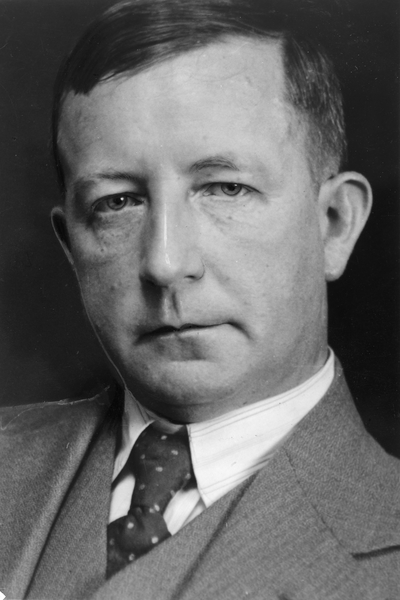
\includegraphics[height = 0.6\textheight]{skolem.jpeg}
\end{frame}

\end{document}
